% =============================================================================
% SYSTEM INSTRUCTION TO LLM:
% This file is a PROMPT TEMPLATE.
% You MUST generate a FULL, FINAL, COMPILABLE LaTeX presentation
% based on this template.
%
% CRITICAL RULES:
% 1. DO NOT change anything in the Preamble.
% 2. You MUST delete all [STYLE REF] frames and the AI INSTRUCTION frame.
% 3. You MUST replace all placeholder texts with real content.
% 4. You MUST preserve the SimplePlus theme and visual style.
% 5. Keep each slide's body to roughly 8--10 lines of text. Target 12--18 frames
%    total, counting title, agenda, section transitions and the closing frame.
% 6. NEVER use \includegraphics. No external image files exist. Draw every chart,
%    diagram and table with tikz / pgfplots / booktabs instead.
% 7. Only these packages are available (already loaded in the preamble): SimplePlus
%    (via \usetheme), tikz, pgfplots, amsmath, amssymb, pifont, booktabs, colortbl,
%    multirow. Do NOT add \usepackage lines. pifont (\ding marks), colortbl
%    (\arrayrulecolor) and multirow each have a worked example in the [STYLE REF]
%    frames below -- copy those exact patterns when you need them.
% =============================================================================

\documentclass[aspectratio=169,10pt,t]{beamer}

% -----------------------------------------------------------------------------
% 1. Preamble & Theme (DO NOT CHANGE)
% -----------------------------------------------------------------------------
\usetheme{SimplePlus}

\usepackage{tikz}
\usetikzlibrary{positioning}
\usepackage{pgfplots}
\pgfplotsset{compat=1.18}
\usepackage{amsmath,amssymb}
\usepackage{pifont}
\usepackage{booktabs}
\usepackage{colortbl}
\usepackage{multirow}

% Auto-generate a highlighted agenda transition at the start of EACH section.
% Just write \section{...} before each section's frames; NEVER hand-type
% agenda or transition frames.
\AtBeginSection[]{%
  \begin{frame}{Agenda}
    \tableofcontents[currentsection,sectionstyle=show/shaded,subsectionstyle=hide]
  \end{frame}
}

% -----------------------------------------------------------------------------
% 2. Metadata (LLM MUST FILL)
% -----------------------------------------------------------------------------
\title[Short Title]{Full Presentation Title}
% Caller fills these three fields. Leave empty when unknown; never invent placeholders.
% Empty fields are safe: the theme skips their boxes on the title page.
\subtitle{}
\author{}
\institute{}
\date{\today}

\begin{document}

% =============================================================================
% FRAME 1: TITLE PAGE (plain: no footer on the opening slide)
% =============================================================================
\begin{frame}[plain,c]
  \titlepage
\end{frame}

% =============================================================================
% FRAME 2: AGENDA
% Filled automatically from your \section{...} commands -- do not hand-type items.
% =============================================================================
\begin{frame}{Agenda}
  \tableofcontents[subsectionstyle=hide]
\end{frame}

% =============================================================================
% SECTION 1 (EXAMPLE)
% Define \section{...} before the first content frame of that section.
% The highlighted agenda transition page is inserted automatically here.
% =============================================================================
\section{First Section Title}

% Content layout 1: text left, figure right
\begin{frame}{Content Example: Text Left, Figure Right}
\small
\begin{columns}[T]
\column{0.55\textwidth}
Write the core analysis on the left.
Use this area for background, problem definition, reasoning, or methodology.
Keep the text dense and conclusion-oriented; avoid vague filler.

\vspace{0.6em}
\textbf{Key Takeaway:}
State the single main point this slide must convey.

\column{0.40\textwidth}
\centering
% Side panel: FEW categories only (4--6 short labels). Compact width. No xlabel.
% For 12-month / many-label series use the full-width chart on the next example page.
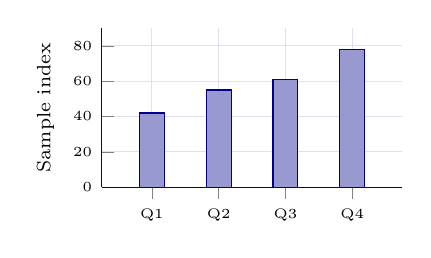
\begin{tikzpicture}
\begin{axis}[
    width=5.4cm,
    height=3.6cm,
    ybar,
    bar width=9pt,
    enlarge x limits=0.25,
    ymin=0, ymax=90,
    symbolic x coords={Q1,Q2,Q3,Q4},
    xtick=data,
    ylabel={Sample index},
    tick label style={font=\tiny},
    label style={font=\scriptsize},
    axis y line*=left,
    axis x line*=bottom,
    axis line style={DarkBlue},
    grid=major,
    grid style={DarkBlue!12},
]
\addplot[fill=DarkBlue!40, draw=DarkBlue] coordinates {
    (Q1,42) (Q2,55) (Q3,61) (Q4,78)
};
\end{axis}
\end{tikzpicture}
\end{columns}
\end{frame}

% =============================================================================
% SECTION 2 (EXAMPLE) -- again, the transition page appears automatically.
% =============================================================================
\section{Second Section Title}

% Content layout 2: text above, figure below
\begin{frame}{Content Example: Text Above, Figure Below}
\small

% Upper text region
When a series has many categories (for example 12 months), use this
full-width layout below -- not the narrow side-panel chart.
Keep the prose short so the wide chart remains readable.

\vspace{1em}

% Lower figure: MANY categories (12 months) → MUST be wide + rotated x labels
\centering
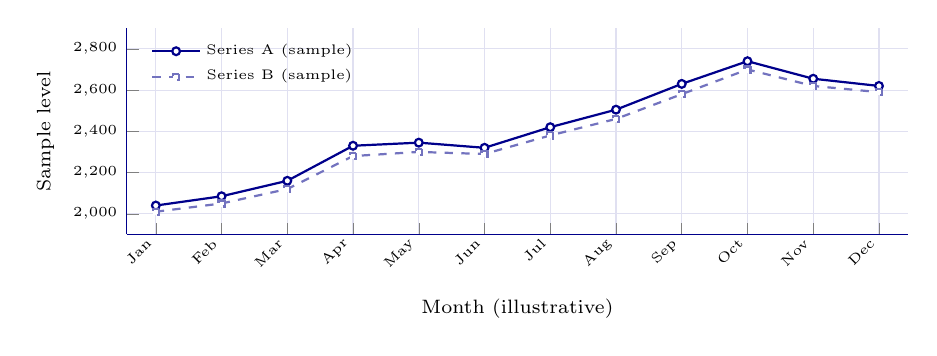
\begin{tikzpicture}
\begin{axis}[
    width=11.5cm, height=4.2cm,
    enlarge x limits=0.04,
    x tick label style={rotate=45, anchor=east, font=\tiny},
    ylabel style={font=\scriptsize},
    xlabel style={font=\scriptsize, yshift=-2pt},
    ymin=1900, ymax=2900,
    symbolic x coords={Jan,Feb,Mar,Apr,May,Jun,Jul,Aug,Sep,Oct,Nov,Dec},
    xtick=data,
    ylabel={Sample level},
    xlabel={Month (illustrative)},
    legend style={at={(0.02,0.98)}, anchor=north west, font=\tiny, draw=none, fill=none},
    yticklabel style={font=\tiny},
    axis y line*=left,
    axis x line*=bottom,
    grid=major,
    grid style={DarkBlue!12},
    axis line style={DarkBlue},
]
\addplot[
    thick,
    mark=*,
    DarkBlue,
    mark options={fill=white, draw=DarkBlue, scale=0.7},
] coordinates {
    (Jan,2040) (Feb,2085) (Mar,2160) (Apr,2330) (May,2345) (Jun,2320)
    (Jul,2420) (Aug,2505) (Sep,2630) (Oct,2740) (Nov,2655) (Dec,2620)
};
\addplot[
    thick,
    dashed,
    DarkBlue!55,
    mark=square*,
    mark options={fill=white, draw=DarkBlue!55, scale=0.55},
] coordinates {
    (Jan,2010) (Feb,2050) (Mar,2120) (Apr,2280) (May,2300) (Jun,2290)
    (Jul,2380) (Aug,2460) (Sep,2580) (Oct,2700) (Nov,2620) (Dec,2590)
};
\legend{Series A (sample), Series B (sample)}
\end{axis}
\end{tikzpicture}

% Add a real source line under the chart only if the source document names one;
% otherwise omit it entirely. Never write generic filler like "compiled from the
% source document".
\end{frame}


% Content layout 3: figure left, text right
\begin{frame}{Content Example: Figure Left, Text Right}
\small
\begin{columns}[c] % [c] vertical center; use [T] for top align if text is long

% Left: real TikZ structure diagram (layered pipeline)
\column{0.45\textwidth}
    \centering
    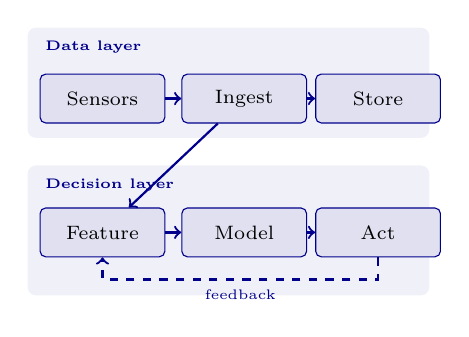
\begin{tikzpicture}[
        font=\scriptsize,
        box/.style={
            draw=DarkBlue, fill=DarkBlue!12, rounded corners=2pt,
            minimum height=0.62cm, text width=1.35cm, align=center
        },
        layer title/.style={font=\tiny\bfseries, text=DarkBlue}
    ]
        % Data layer
        \fill[DarkBlue!6, rounded corners=3pt] (-0.25,1.05) rectangle (4.85,2.45);
        \node[layer title, anchor=north west] at (-0.15,2.40) {Data layer};
        \node[box] (s1) at (0.7,1.55) {Sensors};
        \node[box] (s2) at (2.5,1.55) {Ingest};
        \node[box] (s3) at (4.2,1.55) {Store};
        % Decision layer
        \fill[DarkBlue!6, rounded corners=3pt] (-0.25,-0.95) rectangle (4.85,0.70);
        \node[layer title, anchor=north west] at (-0.15,0.65) {Decision layer};
        \node[box] (p1) at (0.7,-0.15) {Feature};
        \node[box] (p2) at (2.5,-0.15) {Model};
        \node[box] (p3) at (4.2,-0.15) {Act};
        % Edges
        \draw[->, thick, DarkBlue] (s1) -- (s2);
        \draw[->, thick, DarkBlue] (s2) -- (s3);
        \draw[->, thick, DarkBlue] (s2) -- (p1);
        \draw[->, thick, DarkBlue] (p1) -- (p2);
        \draw[->, thick, DarkBlue] (p2) -- (p3);
        \draw[->, thick, DarkBlue, dashed]
            (p3.south) -- ++(0,-0.28) -| (p1.south)
            node[pos=0.25, below, font=\tiny, text=DarkBlue] {feedback};
    \end{tikzpicture}

% Right: analysis region (50% width)
\column{0.50\textwidth}
    \textbf{Object / figure analysis:}

    Interpret the visual on the left. Suitable for:
    \begin{itemize}
        \item Physical structure of equipment
        \item Module-level details of a model
        \item A focused vertical data slice
    \end{itemize}

    \vspace{1em}
    \textbf{Key findings:}
    \begin{enumerate}
        \item \textbf{Observation 1}: The left figure shows...
        \item \textbf{Observation 2}: Relative to expectation, the result...
    \end{enumerate}
\end{columns}
\end{frame}

% =============================================================================
% [STYLE REF] TABLE PAGE (DELETE IN FINAL OUTPUT)
% Shows the worked patterns for booktabs + colortbl + multirow + pifont.
% =============================================================================
\begin{frame}{[STYLE REF] Table Style Example}
\small
\centering
% Zebra striping (\rowcolors) only earns its keep at 5+ data rows; omit it below that.
% Numeric columns right-aligned; \arrayrulecolor ties the rules to the theme.
\renewcommand{\arraystretch}{1.3}
\footnotesize
\arrayrulecolor{DarkBlue!70}
\begin{tabular}{l l r r l}
\toprule
Group & Metric & A & B & Verdict \\
\midrule
\multirow{2}{*}{Quality} & Item one & 12 & 15 & {\color{MediumRed}\ding{55}}~Room to improve \\
 & Item two & 20 & 18 & {\color{MediumGreen}\ding{51}}~Stable \\
\cmidrule(lr){2-5}
Delivery & Item three & 31 & 29 & {\color{MediumGreen}\ding{51}}~On target \\
\bottomrule
\end{tabular}
\end{frame}

% =============================================================================
% [STYLE REF] TIKZ FLOW PAGE (DELETE IN FINAL OUTPUT)
% =============================================================================
\begin{frame}{[STYLE REF] Flowchart Style Example}
\centering
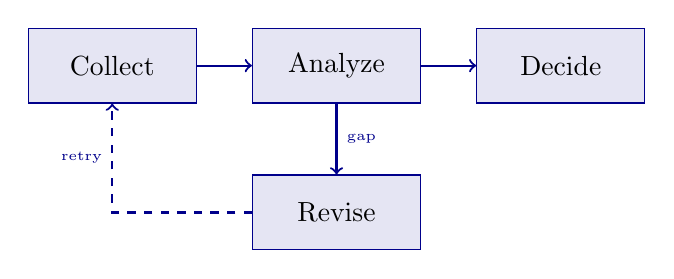
\begin{tikzpicture}[
node distance=0.9cm and 0.7cm,
process/.style={rectangle,draw=DarkBlue,fill=DarkBlue!10,
minimum height=0.95cm,text width=1.9cm,align=center}
]
\node[process] (a) {Collect};
\node[process,right=of a] (b) {Analyze};
\node[process,right=of b] (c) {Decide};
\node[process,below=of b] (d) {Revise};
\draw[->,thick,DarkBlue] (a)--(b);
\draw[->,thick,DarkBlue] (b)--(c);
\draw[->,thick,DarkBlue] (b)--(d)
    node[midway,right,font=\tiny,text=DarkBlue] {gap};
\draw[->,thick,DarkBlue,dashed] (d.west) -| (a.south)
    node[near end,left,font=\tiny,text=DarkBlue] {retry};
\end{tikzpicture}
\end{frame}

% =============================================================================
% [STYLE REF] BLOCKS & EMPHASIS (DELETE IN FINAL OUTPUT)
% The theme's block palette (navy / green / red) plus pifont checklist marks.
% =============================================================================
\begin{frame}{[STYLE REF] Blocks \& Emphasis Example}
\small
\begin{columns}[T]
\column{0.50\textwidth}
\begin{block}{Definition or context}
Use a block for neutral statements: definitions, scope, assumptions.
\end{block}
\begin{exampleblock}{Positive finding}
Use an example block for results that support the recommendation.
\end{exampleblock}
\begin{alertblock}{Risk or caveat}
Use an alert block for warnings, open issues, or hard limits.
\end{alertblock}

\column{0.44\textwidth}
\textbf{Checklist style with pifont:}
\begin{itemize}
    \item[{\color{MediumGreen}\ding{51}}] One takeaway per slide
    \item[{\color{MediumGreen}\ding{51}}] Units and sources on every chart
    \item[{\color{MediumRed}\ding{55}}] Dense paragraphs of prose
    \item[{\color{MediumRed}\ding{55}}] Decorative charts with no message
\end{itemize}
\end{columns}
\end{frame}

% =============================================================================
% AI INSTRUCTION PAGE (DELETE IN FINAL OUTPUT)
% =============================================================================
\begin{frame}[allowframebreaks]{AI GENERATION INSTRUCTIONS}
You MUST:
\begin{itemize}
\item Delete all [STYLE REF] frames and this instruction frame
\item Replace all placeholders with real content
\item Write \texttt{\textbackslash section\{...\}} before the first frame of each
      section; the highlighted agenda transition page is inserted automatically --
      never hand-type agenda or transition frames
\item Use columns layout for all content pages
\item Keep information density high (no empty slides)
\item Target 12--18 frames total
\item Output FULL LaTeX code only
\end{itemize}
\end{frame}

% =============================================================================
% FINAL PAGE
% =============================================================================
\begin{frame}[c]{Thank You}
\centering
{\Large Thank you for your attention.}

\vspace{1.2em}
{\large Questions \& Discussion}

\vspace{1.5em}
% Renders "author | institute" only when that metadata exists; safe when empty.
\SimplePlusClosingAttribution
\end{frame}

\end{document}
